\begin{frame}{Testing setup}
    \begin{figure}
        \centering
        \resizebox{1\textwidth}{!}{
            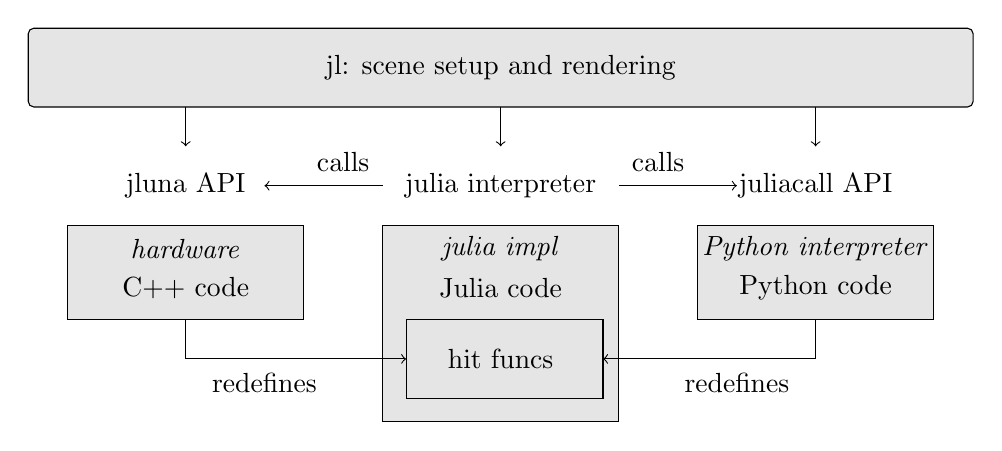
\begin{tikzpicture}
                % beveled 10x4 rectangle with text in the middle "jl: scene setup and rendering"
                \draw[rounded corners=2pt, fill=black!10] (0,0) rectangle (12,1);
                \node at (6,0.5) {jl: scene setup and rendering};
                % arrow down 2 units @ (1.5, 1)
                \draw[->] (2,0) -- (2,-.5);
                \node at (2,-1) {jluna API};
                % draw box 3 wide and 2 tall below node 
                \draw[fill=black!10] (.5,-1.5) rectangle (3.5,-2.7);
                % draw text at top of this box in italics "hardware"
                \node at (2,-1.8) {\textit{hardware}};
                \node at (2, -2.3) {C++ code};
                
                \draw[fill=black!10] (4.5,-1.5) rectangle (7.5,-4);
                \node at (6,-1.8) {\textit{julia impl}};
                \node at (6, -2.3) {Julia code};
                % draw box inside julia code box and inside that write "hit funcs"
                \draw[fill=black!10] (4.8,-2.7) rectangle (7.3,-3.7);
                \node at (6,-3.2) {hit funcs};
                
                % arrow that bends 90 degrees into julia impl from bottom of c++ box 
                \draw[->] (2,-2.7) -- (2,-3.2) -- (4.8,-3.2);
                % add text below arrow that says "redefines"
                \node at (3,-3.5) {redefines};
              
                % arrow down 2 units @ (7.5, 1)
                \draw[->] (10,0) -- (10,-.5);
                \node at (10,-1) {juliacall API};
                % draw box 3 wide and 2 tall below node
                \draw[fill=black!10] (8.5,-1.5) rectangle (11.5,-2.7);
                % draw text at top of this box in italics "julia impl"
                \node at (10,-1.8) {\textit{Python interpreter}};
                \node at (10, -2.3) {Python code};
                
                % arrow that bends 90 degrees into julia impl from bottom of python box
                \draw[->] (10,-2.7) -- (10,-3.2) -- (7.3,-3.2);
                % add text below arrow that says "redefines"
                \node at (9,-3.5) {redefines};
              
                % arrow down in the middle between above 2 
                \draw[->] (6,0) -- (6, -.5);
                \node at (6,-1) {julia interpreter};
                % arrow from julia interpreter to jluna API with the text "calls"
                \draw[->] (4.5,-1) -- (3, -1);
                \node at (4,-.7) {calls};
              
                % arrow from julia interpreter to juliacall API with the text "calls"
                \draw[->] (7.5,-1) -- (9, -1);
                \node at (8,-.7) {calls};
              \end{tikzpicture}
        }
        \caption{Testing setup for component isolation}
    \end{figure}
\end{frame}